% !TeX root = ../solution.tex

\hypertarget{he22.22}{%
\chapter{%
\texorpdfstring{[HE22.22] H$_2$O}{[HE22.22] H2O}}\label{he22.22}}

\begin{marginfigure}
	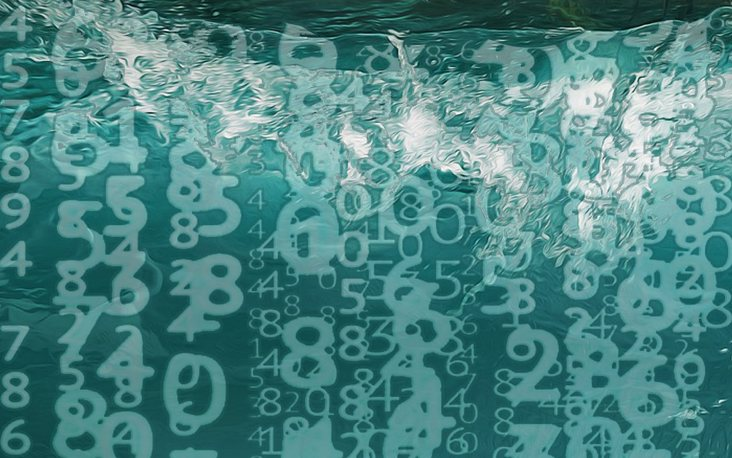
\includegraphics[width=49mm]{level6/challenge22.jpg}
\end{marginfigure}
\section{Intro}
Just some H$_2$O ...

\begin{fullwidth}
\texttt{\noindent
33333336333032303332333333373230333233333330323033323330333032303333333633303
23033323333333732303332333133343230333233313332323033343330323033363336323033
37333032303334333032303336333632303336333532303334333032303336333632303336333
23230333433303230333 63333323033363330323033343330323033363333323033363332323
03334333032303336333632303336333232303334333032303336333732303331333433323230
33343330323033363336323033373330323033343330323033363331323033363337323033363
33132303334333032303336333632303336333432303334333032303336333732303336333232
30333433303230333633363230333633303230333433303230333633363230333633373230333
43330323033363333323033363333323033343330323033363331323033363335323033363336
32303334333032303336333532303331333433363230333433303230333633363230333133343
33532303334333032303336333132303336333332303336333732303334333032303336333332
30333633303230333433303230333633373230333733303230333433303230333633313230333
63337323033363331323033343330323033363336323033363337323033343330323033363333
32303336333332303334333032303336333132303336333532303336333632303334333032303
33633373230333133343334
}
\end{fullwidth}

\section{Solution}\label{hv22.22solution}

It is noticeable that the message contains may threes, and the hint can point
at a conversion from hex to octal representation of numbers.  The ASCII code of
0x33 corresponds to the character `3', so it seems a good idea to convert twice
from hex to character.  Try this using CyberChef and we get a result that
contains packets of octal numbers separated by spaces.  Convert this from octal
to get another string: {\small\texttt{\NotoEmoji 😀🌊} 68 65 62 30 32 62 7b 68 171 64 72 60 67 33
156 5f 6e 137 30 78 171 67 33 156 7d}.

This looks promising, the numbers can again be interpreted as hex and octal
numbers: always two hex numbers, then one octal number.  This then corresponds
to the flag \verb+he2022{hydr0g3n_n_0xyg3n}+:


	









